\chapter{TINJAUAN PUSTAKA}
\label{chap:tinjauanpustaka}

% Ubah bagian-bagian berikut dengan isi dari tinjauan pustaka

\section{Penelitian Terdahulu}
\label{sec:penelitianterdahulu}

\subsection{Kontrol Kursi Roda Menggunakan Sinyal Suara Melalui Bluetooth}

Pada tahun 2023 telah dilakukan penelitian yang berjudul "Kontrol Kursi Roda Menggunakan Sinyal Suara Melalui Bluetooth" oleh Arief Wisaksono, Rachmad Aditya Pratama, dan Hindarto hindarto dari Departemen Teknik Elektro, Fakultas Sains dan Teknologi Universitas Muhammadiyah Sidoarjo \parencite{wisaksono2023kontrol}.

Pada penelitian ini dapat disimpulkan bahwa pengujian koneksi Bluetooth dan Android dapat berjalan secara optimal. Sehingga input dari Android bisa terkirim ke rangkaian Arduino Uno. Hasil pengujian koneksi memiliki waktu delay selama 4 detik hingga 6 detik. Pengujian baterai 12 Volt memiliki deviasi sebesar 0,43 serta akurasi sebesar 96,7\%. Hal ini disebabkan karena hasil dari pengukuran lebih besar daripada tegangan yang diperlukan. Akan tetapi hal tersebut tidak mempengaruhi sistem kerja alat karena tegangan 12 Volt merupakan tegangan minimum alat.

\subsection{Rancang Bangun Kursi Roda Elektrik Dengan Sistem Kontrol \emph{Joystick} Dan \emph{Smartphone} Android}

Pada tahun 2023 telah dilakukan penelitian yang berjudul "Rancang Bangun Kursi Roda Elektrik Dengan Sistem Kontrol \emph{Joystick} dan \emph{Smartphone} Android" oleh Bayu Ahityanto Wicaksono dari Program Studi Diploma IV Rekayasa Perancangan Mekanik, Sekolah Vokasi Universitas Diponegoro \parencite{wicaksono2023rancang}.

Pada penelitian ini didapatkan kesimpulan bahwa kursi roda konvensional yang dijadikan kursi roda elektrik berhasil dijalankan dengan kecepatan maksimal 2 km/h sesuai perencanaan. Kursi roda elektrik dapat dikontrol dengan \emph{joystick} maupun dari aplikasi yang berada di \emph{smartphone} android. Kursi roda elektrik dapat berjalan dengan beban maksimal 80 kg. Terdapat beberapa saran dari penulis seperti menambahkan sandaran kepala agar pengguna lebih nyaman di kursi roda elektrik, serta pembuatan sistem aplikasi untuk pengguna \emph{smartphone} dari Apple.

\subsection{\emph{Wheelchair Control Using Bluetooth-Based Electromyography Signals}}

Telah dilakukan penelitian yang berjudul \emph{"Wheelchair Control Using Bluetooth-Based Electromyography Signals"} oleh Yoga Eko Prasetyo dari Program Studi Teknik Elektro dan Hindarto Hindarto dari Program Studi Informatika Universitas Muhammadiyah Sidoarjo \parencite{prasetyowheelchair}.

Pada penelitian ini didapatkan kesimpulan bahwa durasi tunggu dari bluetooth master dengan bluetooth slave sebesar 4 detik hingga 5 detik. Pengujian sensor elektromiografi dapat berjalan dengan normal dan menghasilkan nilai yang berbeda ketika otot berkontraksi maupun relaksasi. 

\subsection{Prototipe Kursi Roda Elektrik Dengan Kendali \emph{Joystick} dan \emph{Smartphone}}

Pada tahun 2019 telah dilakukan penelitian yang berjudul "Prototipe Kursi Roda Elektrik Dengan Kendali \emph{Joystick} dan \emph{Smartphone}" oleh Andy Sadewa Junior dan Fatchul Arifin dari Program Studi Teknik Elektronika, Fakultas Teknik Universitas Negeri Yogyakarta \parencite{junior2019prototipe}.

Pada penelitian ini didapatkan kesimpulan bahwa total \emph{error} yang dihasilkan dari pengujian tegangan motor kiri dan kanan adalah sebesar 0,144\% dan rata-rata \emph{error} yang didapatkan adalah sebesar 0,024\% pada keseluruhan pengujian yang dilakukan. Pada pengujian bluetooth didapatkan kesimpulan bahwa jangkauan pengiriman optimal dari bluetooth apabila tidak ada penghalang adalah sebesar 1 meter hingga 10 meter.

\subsection{\emph{Vision-based Head Posture Control Wheelchair System Research}}

Pada tahun 2023 telah dilakukan penelitian yang berjudul \emph{"Vision-based Head Posture Control Wheelchair System Research"} oleh Pengyu Gao dari \emph{School of Information Engineering}, \emph{Shenyang University of Chemical Technology} bersama Haitao Luo dan Yuxin Li dari \emph{Department of Space Automation Technology}, \emph{Shenyang Institute of Automation}, \emph{Chinese Academy of Sciences} \parencite{10280784}.

Pada penelitian ini didapatkan kesimpulan bahwa sistem pendeteksi pose kepada berbasis Mediapipe berhasil dilakukan menggunakan metode pemodelan matematis yang dikombinasikan dengan fungsi trigonometri untuk memperkirakan sudut wajah dan arah pose kepala. Namun masih terdapat beberapa \emph{error} pada pengenalan citra karena transmisi input citra bersifat \emph{realtime}.

\section{Teori/Konsep Dasar}

\subsection{\emph{Convolutional Neural Network} (CNN)}

\emph{Convolutional Neural Network} (CNN) telah mencapai hasil yang luar biasa selama beberapa dekade terakhir dalam berbagai bidang yang terkait dengan pengenalan pola, mulai dari pemrosesan gambar hingga pengenalan suara. Aspek paling bermanfaat dari CNN adalah mengurangi jumlah parameter dalam \emph{Artificial Neural Network}. Pencapaian ini telah membantu banyak peneliti dan pengembang dalam mengembangkan model yang lebih besar guna mengatasi tugas-tugas yang kompleks yang tidak mungkin untuk diselesaikan dengan menggunakan \emph{Artificial Neural Network} klasik. Aspek penting dari CNN adalah untuk mendapatkan fitur-fitur abstrak ketika input menyebar menuju lapisan-lapisan yang lebih dalam \parencite{8308186}.

Arsitektur pada CNN terdiri dari tiga bagian, yaitu input, \emph{feature learning}, dan \emph{classification}. \emph{Feature Learning} terdiri dari dua buah \emph{convolution layer} dan dua buah \emph{pooling layer}. Pada \emph{classification} terdiri dari dua \emph{hidden layer} dan satu \emph{output layer}. Arsitektur CNN dapat digambarkan seperti pada Gambar 2.1.

% Gambar 2.1
\begin{figure} [ht] \centering
    % Nama dari file gambar yang diinputkan
    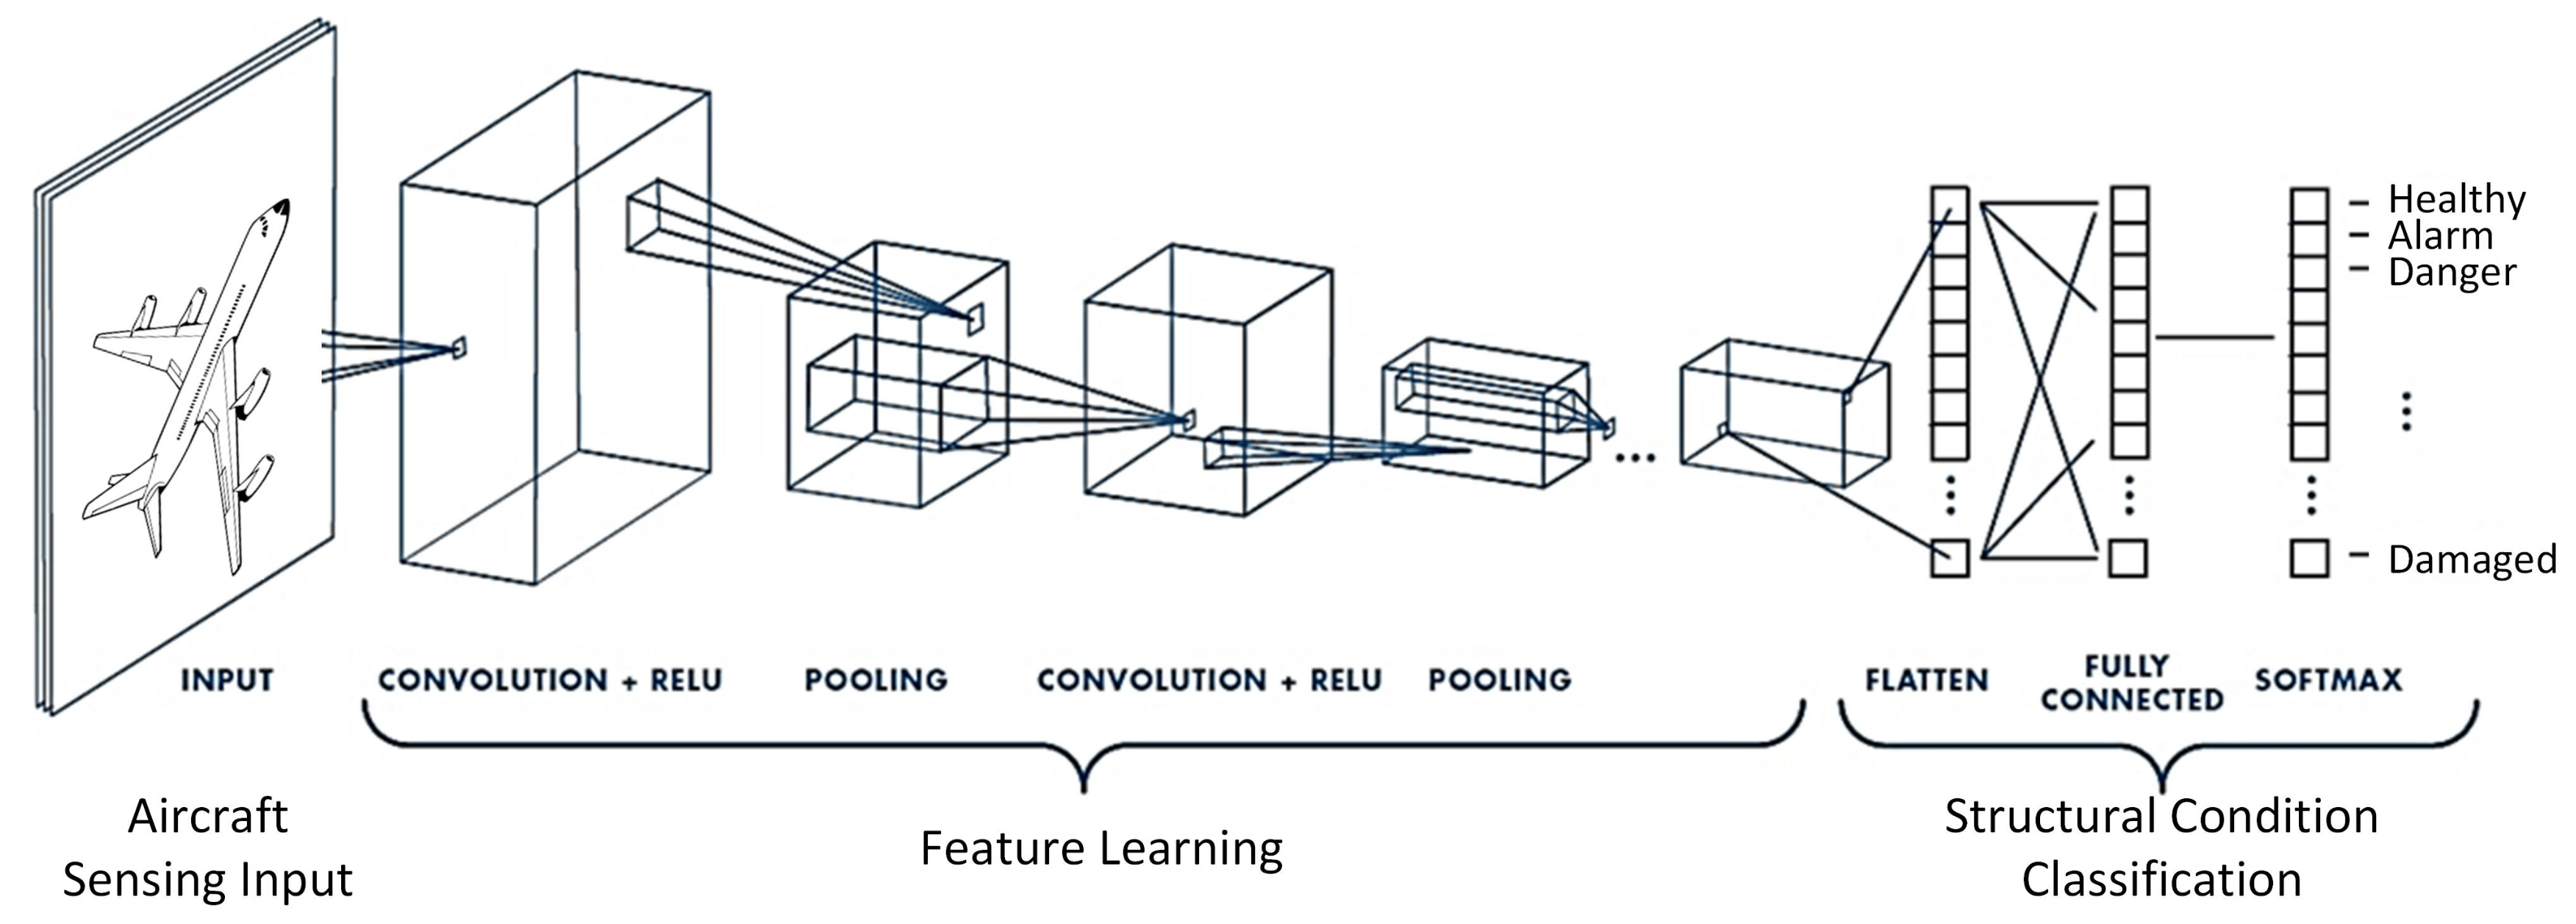
\includegraphics[scale=0.12]{gambar/arsitekturcnn.png}
    % Keterangan gambar yang diinputkan
    \caption{Arsitektur pada \emph{Convolutional Neural Network}}
    % Label referensi dari gambar yang diinputkan
    \label{fig:arsitektur cnn}
\end{figure}

Input CNN merupakan array tiga dimensi dengan ukuran seperti pada Persamaan 2.1. Apabila input merupakan suatu citra maka citra tersebut harus diubah menjadi array dua dimensi. 

% Persamaan 2.1
\begin{equation}
Baris * Kolom * Depth
\end{equation}

\emph{Convolution Layer} digunakan untuk menyaring (\emph{filter}) matriks dari citra \emph{input}. \emph{Zero Padd-ing} akan diperlukan untuk mempertahankan ukuran matriks dari citra \parencite{dwitama2019klasifikasi}. Ukuran kernel yang digunakan pada layer konvolusi adalah \(3 \times 3\) dan \(5 \times 5\). \emph{Output} dari lapisan konvolusi ini akan digunakan sebagai \emph{input} pada \emph{Pooling Layer} \parencite{hakim2018penerapan}. Apabila output dari \emph{Convolution Layer} bernilai negatif maka akan dilakukan perhitungan tambahan berupa aktifasi ReLU. Fungsi aktivasi ReLU akan nilai matriks yang bernilai negatif menjadi nol. Contoh penerapan dari aktivasi ReLU dapat dilihat pada Gambar 2.2.

% Gambar 2.2
\begin{figure} [ht] \centering
    % Nama dari file gambar yang diinputkan
    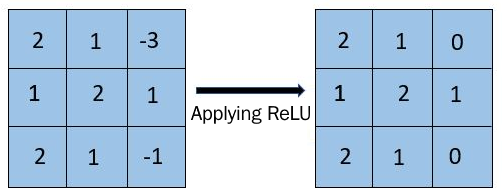
\includegraphics[scale=1]{gambar/aktivasiReLU.png}
    % Keterangan gambar yang diinputkan
    \caption{\emph{Aktivasi ReLU}}
    % Label referensi dari gambar yang diinputkan
    \label{fig:Aktivasi ReLU}
\end{figure}

\emph{Pooling Layer} digunakan untuk mengurangi jumlah parameter ketika ukuran citra terlalu besar dengan cara mengurangi dimensi setiap fitur. Karena ukuran citra menjadi lebih kecil maka proses \emph{feature map} akan menjadi lebih cepat \parencite{hakim2018penerapan}. \emph{Max Pooling} dilakukan dengan cara mengambil nilai dengan elemen terbesar sesuai dengan ukuran filter. Sebagai contoh pada Gambar 2.3 merupakan \emph{max pooling} dengan filter \(2 \times 2\) dengan \emph{stride} sebesar 2.

% Gambar 2.3
\begin{figure} [ht] \centering
    % Nama dari file gambar yang diinputkan
    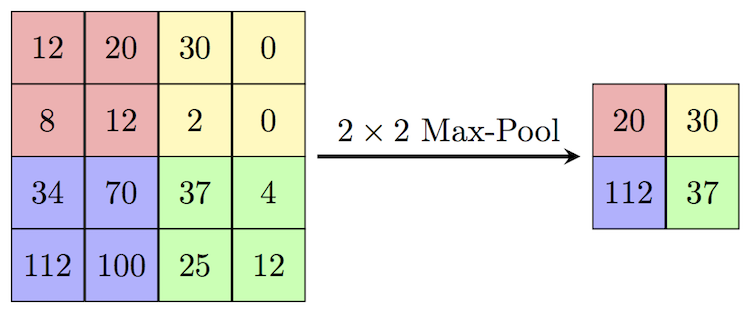
\includegraphics[scale=1.5]{gambar/maxPooling.png}
    % Keterangan gambar yang diinputkan
    \caption{\emph{Max Pooling}}
    % Label referensi dari gambar yang diinputkan
    \label{fig:Max Pooling}
\end{figure}

Flatten merupakan suatu proses dimana hasil dari \emph{Feature Learning} diubah menjadi vektor yang selanjutnya akan menjadi input pada proses klasifikasi dengan arsitektur \emph{fully connected layer}. Flatten digunakan untuk mengubah matriks menjadi vektor dengan menyesuaikan sesuai format \emph{input} pada \emph{neural network layer}. Flatten dapat digambarkan seperti pada Gambar 2.4.

% Gambar 2.4
\begin{figure} [ht] \centering
    % Nama dari file gambar yang diinputkan
    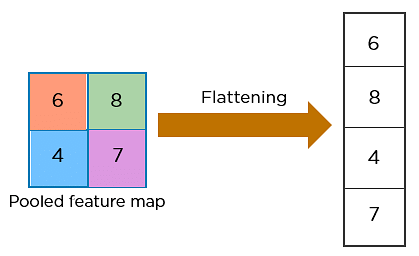
\includegraphics[scale=0.6]{gambar/flattening.png}
    % Keterangan gambar yang diinputkan
    \caption{Proses \emph{Flattening}}
    % Label referensi dari gambar yang diinputkan
    \label{fig:Proses Flattening}
\end{figure}

\newpage

\subsection{NVIDIA® Jetson Nano™}

% Gambar 2.1
\begin{figure} [ht] \centering
    % Nama dari file gambar yang diinputkan
    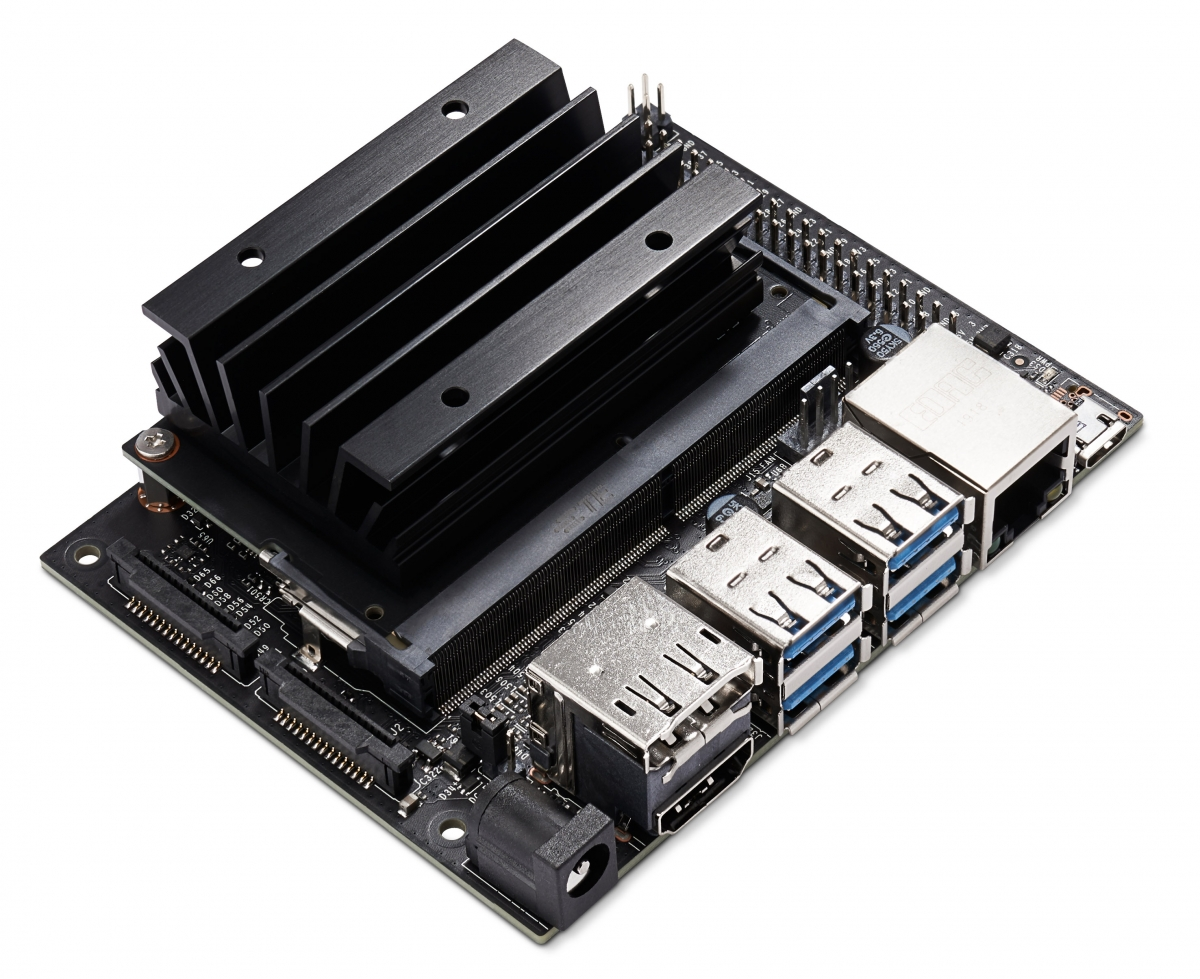
\includegraphics[scale=0.25]{gambar/JetsonNano.jpg}
    % Keterangan gambar yang diinputkan
    \caption{Perangkat Jetson Nano}
    % Label referensi dari gambar yang diinputkan
    \label{fig:Perangkat Jetson Nano}
\end{figure}

NVIDIA® Jetson Nano™ Developer Kit adalah komputer kecil dan kuat yang dapat digunakan untuk menjalankan beberapa \emph{neural network} secara paralel untuk berbagai penerapan seperti klasifikasi gambar, deteksi objek, segmentasi, dan pemrosesan ucapan. Semuanya dikemas dalam platform yang mudah digunakan dan hanya membutuhkan daya 5 watt \parencite{Developer_2023}.

Perangkat ini memiliki pin \emph{input} serta \emph{output} yang berlimpah, mulai dari GPIO hingga pin CSI. Jumlah pin yang berlimpah ini sangat memudahkan para pengembang dalam menghubung-kan berbagai perangkat tambahan seperti sensor untuk keperluan pengembangan aplikasi \emph{Artificial Intelligence}. NVIDIA® Jetson Nano™ Developer Kit juga didukung dengan NVIDIA JetPack yang mencakup berbagai perangkat lunak seperti Sistem Operasi Linux, cuDNN, NVIDIA CUDA, TensorRT, dan juga \emph{Board Support Package} (BSP) yang digunakan untuk keperluan \emph{Deep Learning} serta visi komputer.